% !TEX root = main.tex
\documentclass[conference]{IEEEtran}
% --- IEEE Conference Preamble ---
\usepackage[utf8]{inputenc}
\usepackage[T1]{fontenc}

\usepackage{amsmath, amssymb}
\usepackage{graphicx}
\usepackage{booktabs}
\usepackage{array}
\usepackage{tabularx}
\usepackage{tikz}
\usetikzlibrary{arrows.meta, positioning, shapes.geometric}
\usepackage{xcolor}
\usepackage{hyperref}
\hypersetup{
    colorlinks=true,
    linkcolor=black,
    citecolor=blue!70!black,
    urlcolor=blue!70!black,
}
\usepackage{cite}


\begin{document}

\title{Pemodelan Peto's Paradox melalui Regulasi Siklus Sel dalam Supresi Risiko Kanker}

\author{
\IEEEauthorblockN{
Mochammad Fariz Rifqi Rizqulloh\textsuperscript{1},
Muhammad Jibril Ibrahim\textsuperscript{2},
Nayaka Ghana Subrata\textsuperscript{3}}
\IEEEauthorblockA{
Program Studi Teknik Informatika,
Sekolah Teknik Elektro dan Informatika\\
Institut Teknologi Bandung, Bandung, Indonesia\\
\textsuperscript{1}13523069@std.stei.itb.ac.id,
\textsuperscript{2}13523085@std.stei.itb.ac.id,
\textsuperscript{3}13523090@std.stei.itb.ac.id}
}

\maketitle

\begin{abstract}
Kanker muncul ketika sel dengan kerusakan genetik lolos dari kontrol siklus
sel dan terus membelah. Secara intuitif, organisme besar dan berumur
panjang diperkirakan memiliki risiko kanker lebih tinggi karena memiliki
lebih banyak sel dan lebih banyak kesempatan akumulasi mutasi. Namun,
Peto's Paradox menunjukkan bahwa risiko kanker antarspesies tidak meningkat
secara proporsional terhadap ukuran tubuh. Paper ini menganalisis paradoks
tersebut menggunakan dataset kanker lintas mamalia dari Vincze dkk.,
yang memuat cancer mortality risk, massa tubuh, adult life expectancy,
jumlah catatan postmortem, dan kasus neoplasia. Setelah filtering nilai
kosong, 172 spesies dianalisis. Regresi log massa tubuh terhadap
log CMR menghasilkan slope -0{,}086 dengan $R^2=0{,}053$, sedangkan
exposure proxy massa tubuh dikali adult life expectancy menghasilkan slope
-0{,}063 dengan $R^2=0{,}034$. Hasil ini menunjukkan bahwa
skala tubuh dan umur menjelaskan sebagian kecil variasi CMR. Kami
kemudian membangun residual supresi berbasis risiko naif untuk
mengidentifikasi spesies dengan CMR lebih rendah daripada prediksi exposure.
Residual tersebut ditafsirkan sebagai kandidat sinyal mekanisme supresi
kanker, termasuk DNA repair, checkpoint, dan apoptosis.
\end{abstract}

\begin{IEEEkeywords}
Peto's Paradox, siklus sel, DNA repair, checkpoint, apoptosis,
comparative oncology, cancer mortality risk
\end{IEEEkeywords}

\section{Pendahuluan}

Kanker muncul ketika sel yang membawa perubahan genetik atau epigenetik
memperoleh kemampuan untuk membelah, bertahan hidup, dan berekspansi secara
tidak normal. Pada tingkat sel, proses ini berkaitan dengan akumulasi mutasi,
kegagalan DNA repair, checkpoint yang tidak cukup menahan pembelahan, dan
apoptosis yang tidak berhasil mengeliminasi sel berisiko
\cite{hanahan2022,alberts2015}. Karena itu, risiko kanker tidak hanya dapat
dibaca sebagai masalah ukuran organisme, tetapi juga sebagai hasil dinamika
populasi sel. Dengan fokus pada pembelahan sel, checkpoint, akumulasi mutasi,
dan eliminasi sel rusak, proyek ini ditempatkan dalam topik siklus sel.

Secara intuitif, organisme yang lebih besar dan hidup lebih lama diperkirakan
memiliki risiko kanker lebih tinggi. Mereka memiliki lebih banyak sel dan lebih
banyak kesempatan pembelahan sepanjang hidup. Namun, Peto's Paradox
menyatakan bahwa risiko kanker antarspesies tidak meningkat secara
proporsional terhadap ukuran tubuh dan umur \cite{peto1977,caulin2011}.
Paradoks ini mengarah pada pertanyaan mekanistik: mekanisme apa yang dapat
mengurangi peluang sel kanker muncul atau lolos dari kontrol organisme besar?

Studi ini menempatkan simulasi sebagai kontribusi utama. Kami membangun model
populasi sel yang merepresentasikan sel sehat, termutasi, prakanker, dan
kanker. Model ini menguji bagaimana pembelahan, mutasi, repair, apoptosis,
jumlah mutasi yang dibutuhkan untuk transformasi, serta kontrol imun
memengaruhi cancer escape. Dalam laporan ini, cancer escape tidak berarti
kanker klinis pada organisme nyata, melainkan kondisi operasional dalam simulasi
ketika jumlah unit sel kanker melampaui ambang kontrol imun.

Analisis dataset mamalia dari Vincze dkk. \cite{vincze2022} digunakan sebagai
konteks empiris. Dataset tersebut memuat adult cancer mortality risk (CMR),
incidence of cancer mortality (ICM), massa tubuh, adult life expectancy, jumlah
individu, jumlah catatan postmortem, dan jumlah kasus neoplasia. Analisis ini
menunjukkan apakah pola data nyata mendukung motivasi dasar simulasi: ukuran
tubuh dan umur saja tidak cukup untuk menjelaskan variasi risiko kanker.

Pertanyaan penelitian yang diajukan adalah:
\begin{enumerate}
    \item Bagaimana model populasi sel sederhana dapat menerjemahkan mutasi
          multi-hit, repair, apoptosis, dan kontrol imun menjadi cancer escape?
    \item Apakah skenario organisme besar dan berumur panjang tanpa mekanisme
          kompensasi menghasilkan escape probability lebih tinggi daripada
          skenario dengan perlindungan biologis?
    \item Bagaimana hasil simulasi tersebut dibaca bersama analisis empiris CMR
          lintas mamalia dari dataset Vincze dkk.?
\end{enumerate}

Kontribusi studi ini adalah kerangka eksplorasi yang menghubungkan teori
biologi kanker dengan pola Peto's Paradox. Model tidak dimaksudkan untuk
memprediksi risiko kanker spesies tertentu. Tujuannya adalah menunjukkan secara
terkendali bagaimana mekanisme yang termotivasi secara biologis dapat
menurunkan cancer escape pada kondisi ukuran dan umur yang lebih besar.

\section{Kajian Pustaka}

\subsection{Peto's Paradox}

Peto's Paradox berangkat dari ketidaksesuaian antara prediksi sederhana dan
data lintas spesies. Jika setiap sel memiliki peluang yang sama untuk
mengalami transformasi kanker, maka organisme besar dan berumur panjang
diperkirakan memiliki risiko kanker lebih tinggi daripada organisme
kecil. Pada kenyataannya, korelasi tersebut lemah atau tidak proporsional
antarspesies \cite{caulin2011}. Hal ini berbeda dengan pola dalam satu
spesies, di mana ukuran tubuh atau umur sering berkaitan dengan risiko
kanker yang lebih tinggi.

Penjelasan biologis yang umum diajukan adalah evolusi mekanisme supresi
kanker. Mekanisme tersebut dapat berupa DNA repair yang lebih efisien,
checkpoint yang lebih ketat, apoptosis yang lebih sensitif, pembatasan
pembelahan stem cell, arsitektur jaringan yang membatasi ekspansi klon,
atau sistem imun yang lebih efektif. Contoh yang banyak dibahas adalah
gajah. Sulak dkk. melaporkan ekspansi salinan TP53 pada gajah dan respons
kerusakan DNA yang lebih aktif \cite{sulak2016}. Tollis dkk. juga melaporkan
percepatan evolusi pada mekanisme pertahanan penyakit gajah
\cite{tollis2021}.

\subsection{Dataset Kanker Lintas Mamalia}

Vincze dkk. menyusun basis data cancer-related mortality pada mamalia dewasa
di bawah perawatan manusia \cite{vincze2022}. Data berasal dari Species360
dan Zoological Information Management System. Analisis utama mereka
melibatkan 191 spesies mamalia dan menunjukkan bahwa cancer mortality risk
sebagian besar independen dari massa tubuh dan adult life expectancy.
Mereka juga menekankan perbedaan antarordo dan kaitan diet dengan risiko
kanker.

Dalam paper ini, data yang tersedia publik dari GitHub penulis digunakan
sebagai input analisis. Kolom utama yang dipakai adalah Species, Order,
Species body mass, Adult life expectancy, CMR, ICM, jumlah individu, jumlah
catatan postmortem, dan jumlah kasus neoplasia. Setelah baris dengan nilai
inti kosong dikeluarkan, analisis menghasilkan 172 spesies. Dari jumlah
tersebut, 131 spesies memiliki CMR lebih dari nol.

\subsection{Siklus Sel sebagai Interpretasi Mekanistik}

Data komparatif tidak mengukur DNA repair, checkpoint, atau apoptosis secara
langsung pada setiap spesies. Karena itu, paper ini tidak mengklaim bahwa
residual statistik adalah indikator langsung satu mekanisme molekuler tertentu.
Sebaliknya, residual dipakai sebagai sinyal komputasional: jika suatu
spesies memiliki exposure proxy tinggi tetapi CMR rendah, maka spesies
tersebut menjadi kandidat untuk diteliti mekanisme supresinya.

Interpretasi siklus sel tetap relevan karena sebagian besar mekanisme
supresi kanker bekerja dengan mengurangi peluang mutasi bertahan dan
berekspansi. DNA repair menurunkan mutasi efektif. Checkpoint menghambat
kelanjutan siklus sel saat kerusakan terdeteksi. Apoptosis menghilangkan
sel berisiko. Dengan demikian, analisis komparatif dapat digunakan untuk
menentukan spesies atau ordo yang layak diprioritaskan dalam studi mekanisme
kontrol siklus sel.

\section{Metode}

\begin{figure}[t]
    \centering
    \resizebox{0.78\columnwidth}{!}{%
    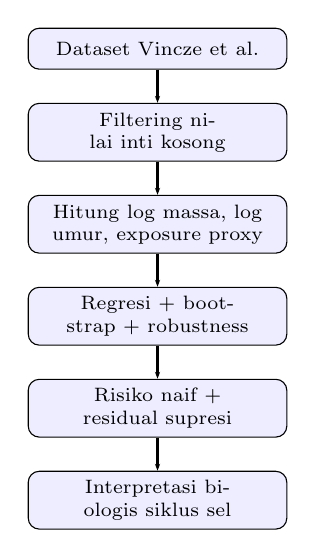
\begin{tikzpicture}[
        node distance=0.42cm,
        block/.style={rectangle, draw, rounded corners, fill=blue!7,
                      minimum height=0.52cm, text width=3.05cm,
                      align=center, font=\scriptsize},
        arr/.style={-{Stealth[length=2.5pt]}, thick}
    ]
        \node[block] (data) {Dataset Vincze et al.};
        \node[block, below=of data] (filter) {Filtering nilai inti kosong};
        \node[block, below=of filter] (features) {Hitung log massa, log umur, exposure proxy};
        \node[block, below=of features] (reg) {Regresi + bootstrap + robustness};
        \node[block, below=of reg] (resid) {Risiko naif + residual supresi};
        \node[block, below=of resid] (bio) {Interpretasi biologis siklus sel};
        \draw[arr] (data) -- (filter);
        \draw[arr] (filter) -- (features);
        \draw[arr] (features) -- (reg);
        \draw[arr] (reg) -- (resid);
        \draw[arr] (resid) -- (bio);
    \end{tikzpicture}}
    \caption{Bagan alir metode komputasi. Analisis bergerak dari dataset
    komparatif menuju regresi, uji robustness, model risiko naif, dan
    interpretasi mekanistik.}
    \label{fig:method-flow}
\end{figure}

\subsection{Data dan Filtering}

Data utama adalah \texttt{SupplementaryData.xls} dari Vincze dkk.
\cite{vincze2022}, diunduh dari repositori GitHub penulis dan dikonversi
menjadi CSV. Dataset memuat spesies mamalia, ordo, massa tubuh, adult life
expectancy, CMR, ICM, jumlah individu, jumlah individu mati, jumlah kasus
neoplasia, dan jumlah catatan postmortem. Baris dengan nilai kosong pada
massa tubuh, adult life expectancy, CMR, atau ICM dikeluarkan. Semua analisis
berikutnya menggunakan 172 spesies yang lolos filtering.

Kode Python tersedia pada repositori proyek:
\url{https://github.com/Nayekah/KDS}. Implementasi memakai pustaka standar
Python agar analisis dapat dijalankan tanpa instalasi paket numerik eksternal.
Komponen program terdiri dari pembaca data, fungsi statistik, analisis
komparatif, dan generator tabel/figur untuk laporan.

% Generated by python main.py
\begin{table}[t]
\centering
\caption{Ringkasan empiris dataset mamalia sebagai konteks Peto's Paradox.}
\label{tab:empirical-context}
\begin{tabular}{lr}
\toprule
Besaran & Nilai\\
\midrule
Jumlah spesies & 172\\
Spesies CMR $>$ 0 & 131\\
Slope log massa--log CMR & -0.086\\
$R^2$ log massa--log CMR & 0.053\\
Slope exposure--log CMR & -0.063\\
$R^2$ exposure--log CMR & 0.034\\
\bottomrule
\end{tabular}
\end{table}

\newcommand{\SpeciesCount}{172}
\newcommand{\NonzeroSpeciesCount}{131}
\newcommand{\MassSlope}{-0.086}
\newcommand{\MassRsq}{0.053}
\newcommand{\ExposureSlope}{-0.063}
\newcommand{\ExposureRsq}{0.034}

CMR digunakan sebagai variabel risiko utama karena merepresentasikan
probabilitas kematian terkait kanker pada individu dewasa. Adult life
expectancy dikonversi dari hari menjadi tahun. Massa tubuh digunakan dalam
kilogram. Untuk mengurangi efek skala yang lebar, hubungan statistik
dihitung pada skala logaritmik untuk massa tubuh, adult life expectancy,
exposure proxy, dan CMR nonnol.

\subsection{Exposure Proxy}

Risiko kanker secara teoritis meningkat dengan jumlah sel dan lama paparan
waktu. Karena jumlah sel aktual tidak tersedia untuk semua spesies, massa
tubuh digunakan sebagai proksi jumlah sel. Exposure proxy didefinisikan
sebagai
\begin{equation}
    E_i = M_i \times L_i,
\end{equation}
dengan $M_i$ adalah massa tubuh spesies $i$ dan $L_i$ adalah adult life
expectancy dalam tahun. Proksi ini tidak mengukur jumlah pembelahan aktual,
tetapi cukup untuk menguji prediksi dasar Peto's Paradox: spesies dengan
$E$ besar diperkirakan memiliki risiko kanker lebih tinggi jika tidak ada
kompensasi biologis.

\subsection{Regresi Skala Tubuh dan Risiko}

Analisis pertama menghitung regresi linear sederhana:
\begin{equation}
    \log_{10}(\mathrm{CMR}_i) =
    \alpha + \beta \log_{10}(X_i) + \epsilon_i,
\end{equation}
dengan $X_i$ berupa massa tubuh, adult life expectancy, atau exposure proxy.
Hanya spesies dengan CMR lebih dari nol yang digunakan dalam regresi log.
Nilai slope dan $R^2$ dilaporkan untuk melihat apakah risiko kanker
meningkat searah dengan ukuran tubuh dan umur.

Untuk menguji kestabilan slope, bootstrap dilakukan 1000 kali dengan
resampling spesies ber-CMR nonnol. Dari distribusi slope bootstrap diambil
rerata dan interval kepercayaan 95\%. Selain itu, regresi massa tubuh
diulang setelah menerapkan ambang minimum catatan postmortem 20, 50, dan
100. Uji ini digunakan karena CMR pada spesies dengan sedikit catatan
postmortem lebih rentan terhadap noise pencatatan.

\subsection{Model Risiko Naif dan Residual Supresi}

Untuk menafsirkan deviasi dari prediksi naif, risiko berbasis exposure
didefinisikan sebagai
\begin{equation}
    R_i^\mathrm{naif} = 1 - \exp(-\lambda E_i).
\end{equation}
Parameter $\lambda$ dikalibrasi sehingga median risiko naif mendekati median
CMR nonnol. Residual supresi kemudian dihitung sebagai
\begin{equation}
    S_i = 1 -
    \frac{-\ln(1-\mathrm{CMR}_i)}{\lambda E_i}.
\end{equation}
Nilai $S_i$ tinggi menunjukkan CMR teramati lebih rendah daripada risiko naif
yang diprediksi oleh exposure proxy. Nilai ini bukan pengukuran langsung
DNA repair atau apoptosis, tetapi kandidat sinyal supresi kanker relatif
yang dapat dikaitkan dengan mekanisme kontrol siklus sel.

\subsection{Ringkasan Ordo}

Selain analisis spesies, data diringkas per ordo. Ordo dengan kurang dari
tiga spesies dikeluarkan dari ringkasan agar median tidak terlalu rapuh.
Untuk setiap ordo dihitung median CMR, median massa tubuh, median adult life
expectancy, dan jumlah spesies. Ringkasan ini digunakan untuk melihat
apakah perbedaan risiko lebih tampak pada tingkat taksonomi daripada pada
skala tubuh saja.

\subsection{Kriteria Interpretasi}

Hasil kuantitatif ditafsirkan dalam tiga tingkat. Pertama, slope regresi
digunakan untuk menjawab apakah ukuran tubuh, umur, atau exposure proxy
memiliki hubungan arah yang konsisten dengan CMR. Kedua, bootstrap dan filtering
postmortem digunakan untuk menilai apakah kesimpulan tersebut stabil
terhadap sampling spesies dan kualitas catatan. Ketiga, residual supresi
digunakan sebagai analisis kualitatif untuk memilih spesies kandidat.
Dengan pemisahan ini, paper tidak menyamakan korelasi statistik dengan
mekanisme biologis langsung, tetapi menggunakan hasil komputasi sebagai
dasar formulasi hipotesis biologis yang lebih terarah.

\section{Hasil dan Diskusi}

\subsection{Konteks Empiris dari Data Mamalia}

Analisis dataset Vincze dkk. menghasilkan \SpeciesCount{} spesies setelah
filtering, dengan \NonzeroSpeciesCount{} spesies memiliki CMR nonnol. Ringkasan
empiris pada Tabel~\ref{tab:empirical-context} menunjukkan bahwa hubungan
antara ukuran tubuh dan risiko kanker lemah: regresi log massa tubuh terhadap
log CMR memiliki slope \MassSlope\ dan $R^2=\MassRsq$, sedangkan exposure proxy
memiliki slope \ExposureSlope\ dan $R^2=\ExposureRsq$. Hasil ini mendukung
motivasi Peto's Paradox: massa tubuh dan umur saja belum cukup untuk
menjelaskan variasi risiko kanker antarspesies.

\begin{figure}[t]
    \centering
    \resizebox{0.92\columnwidth}{!}{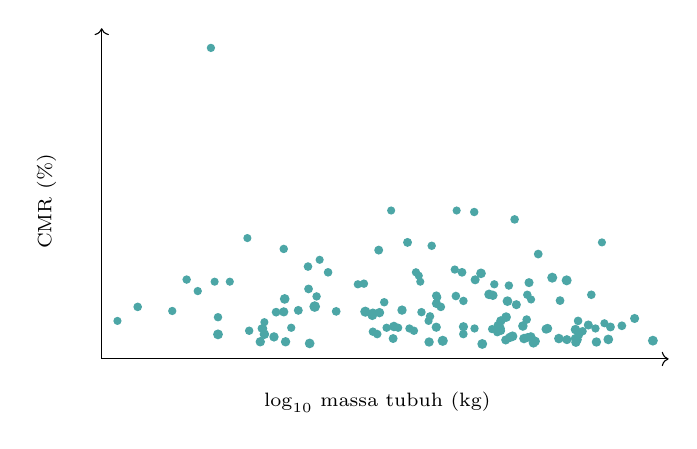
\begin{tikzpicture}[x=1cm,y=1cm]
\draw[->] (0,0) -- (7.2,0);
\draw[->] (0,0) -- (0,4.2);
\node[font=\scriptsize] at (3.5,-0.55) {$\log_{10}$ massa tubuh (kg)};
\node[font=\scriptsize,rotate=90] at (-0.7,2) {CMR (\%)};
\fill[teal!70] (5.057,0.387) circle (0.064);
\fill[teal!70] (5.663,0.387) circle (0.059);
\fill[teal!70] (5.136,0.531) circle (0.062);
\fill[teal!70] (3.814,0.620) circle (0.060);
\fill[teal!70] (5.349,0.418) circle (0.061);
\fill[teal!70] (4.833,0.190) circle (0.063);
\fill[teal!70] (5.070,0.358) circle (0.054);
\fill[teal!70] (3.437,0.556) circle (0.063);
\fill[teal!70] (4.484,1.135) circle (0.053);
\fill[teal!70] (3.991,1.100) circle (0.053);
\fill[teal!70] (5.266,0.689) circle (0.058);
\fill[teal!70] (4.958,0.379) circle (0.053);
\fill[teal!70] (6.768,0.514) circle (0.058);
\fill[teal!70] (6.606,0.421) circle (0.056);
\fill[teal!70] (6.050,0.483) circle (0.055);
\fill[teal!70] (6.271,0.387) circle (0.053);
\fill[teal!70] (2.312,0.598) circle (0.059);
\fill[teal!70] (2.188,0.280) circle (0.060);
\fill[teal!70] (2.066,0.314) circle (0.061);
\fill[teal!70] (2.215,0.594) circle (0.056);
\fill[teal!70] (4.731,1.866) circle (0.054);
\fill[teal!70] (5.131,0.241) circle (0.058);
\fill[teal!70] (5.032,0.427) circle (0.056);
\fill[teal!70] (4.262,0.783) circle (0.052);
\fill[teal!70] (1.477,0.312) circle (0.063);
\fill[teal!70] (4.046,0.981) circle (0.052);
\fill[teal!70] (5.363,0.259) circle (0.061);
\fill[teal!70] (4.743,1.005) circle (0.058);
\fill[teal!70] (4.249,0.403) circle (0.059);
\fill[teal!70] (6.022,0.212) circle (0.060);
\fill[teal!70] (1.850,1.535) circle (0.052);
\fill[teal!70] (1.873,0.358) circle (0.054);
\fill[teal!70] (4.576,1.100) circle (0.056);
\fill[teal!70] (2.729,0.794) circle (0.054);
\fill[teal!70] (5.218,0.288) circle (0.062);
\fill[teal!70] (5.405,0.815) circle (0.054);
\fill[teal!70] (3.444,0.346) circle (0.054);
\fill[teal!70] (1.387,3.950) circle (0.053);
\fill[teal!70] (0.457,0.661) circle (0.055);
\fill[teal!70] (1.477,0.530) circle (0.054);
\fill[teal!70] (6.014,0.259) circle (0.057);
\fill[teal!70] (6.461,0.406) circle (0.057);
\fill[teal!70] (6.107,0.352) circle (0.054);
\fill[teal!70] (6.283,0.215) circle (0.060);
\fill[teal!70] (4.170,0.541) circle (0.054);
\fill[teal!70] (4.594,0.409) circle (0.059);
\fill[teal!70] (3.253,0.948) circle (0.053);
\fill[teal!70] (3.330,0.956) circle (0.054);
\fill[teal!70] (3.499,0.316) circle (0.055);
\fill[teal!70] (4.307,0.661) circle (0.055);
\fill[teal!70] (7.000,0.232) circle (0.063);
\fill[teal!70] (6.040,0.244) circle (0.058);
\fill[teal!70] (5.153,0.734) circle (0.062);
\fill[teal!70] (4.498,0.799) circle (0.055);
\fill[teal!70] (0.896,0.609) circle (0.053);
\fill[teal!70] (5.908,0.245) circle (0.058);
\fill[teal!70] (5.483,0.204) circle (0.061);
\fill[teal!70] (5.427,0.969) circle (0.058);
\fill[teal!70] (0.200,0.483) circle (0.052);
\fill[teal!70] (3.348,0.600) circle (0.065);
\fill[teal!70] (2.497,0.617) circle (0.057);
\fill[teal!70] (4.191,1.437) circle (0.054);
\fill[teal!70] (4.250,0.802) circle (0.056);
\fill[teal!70] (4.735,0.387) circle (0.053);
\fill[teal!70] (4.027,1.057) circle (0.052);
\fill[teal!70] (4.817,1.087) circle (0.062);
\fill[teal!70] (4.594,0.737) circle (0.054);
\fill[teal!70] (3.908,0.387) circle (0.053);
\fill[teal!70] (4.251,0.704) circle (0.058);
\fill[teal!70] (4.061,0.594) circle (0.054);
\fill[teal!70] (4.986,0.948) circle (0.053);
\fill[teal!70] (4.331,0.230) circle (0.065);
\fill[teal!70] (4.920,0.820) circle (0.062);
\fill[teal!70] (3.701,0.259) circle (0.057);
\fill[teal!70] (2.050,0.387) circle (0.053);
\fill[teal!70] (2.066,0.467) circle (0.052);
\fill[teal!70] (1.079,1.008) circle (0.054);
\fill[teal!70] (2.978,0.604) circle (0.056);
\fill[teal!70] (4.158,0.215) circle (0.060);
\fill[teal!70] (2.620,1.173) circle (0.055);
\fill[teal!70] (2.627,0.889) circle (0.056);
\fill[teal!70] (3.765,0.396) circle (0.053);
\fill[teal!70] (5.185,0.274) circle (0.060);
\fill[teal!70] (3.711,0.412) circle (0.061);
\fill[teal!70] (4.508,1.885) circle (0.052);
\fill[teal!70] (2.312,1.397) circle (0.054);
\fill[teal!70] (5.806,0.259) circle (0.061);
\fill[teal!70] (3.588,0.720) circle (0.054);
\fill[teal!70] (3.676,1.885) circle (0.052);
\fill[teal!70] (5.905,0.998) circle (0.064);
\fill[teal!70] (5.244,1.772) circle (0.055);
\fill[teal!70] (5.069,0.483) circle (0.060);
\fill[teal!70] (5.722,1.032) circle (0.064);
\fill[teal!70] (4.968,0.808) circle (0.060);
\fill[teal!70] (4.593,0.316) circle (0.055);
\fill[teal!70] (1.220,0.862) circle (0.053);
\fill[teal!70] (5.544,1.332) circle (0.056);
\fill[teal!70] (5.453,0.755) circle (0.052);
\fill[teal!70] (5.409,0.273) circle (0.057);
\fill[teal!70] (3.618,0.396) circle (0.053);
\fill[teal!70] (4.151,0.483) circle (0.052);
\fill[teal!70] (3.444,0.582) circle (0.059);
\fill[teal!70] (3.884,1.480) circle (0.057);
\fill[teal!70] (2.407,0.396) circle (0.053);
\fill[teal!70] (2.014,0.218) circle (0.060);
\fill[teal!70] (2.768,1.259) circle (0.052);
\fill[teal!70] (5.171,0.932) circle (0.054);
\fill[teal!70] (5.644,0.379) circle (0.059);
\fill[teal!70] (1.434,0.981) circle (0.052);
\fill[teal!70] (5.507,0.224) circle (0.059);
\fill[teal!70] (5.024,0.340) circle (0.054);
\fill[teal!70] (2.335,0.218) circle (0.060);
\fill[teal!70] (2.324,0.762) circle (0.062);
\fill[teal!70] (2.641,0.197) circle (0.062);
\fill[teal!70] (2.032,0.387) circle (0.053);
\fill[teal!70] (3.965,0.358) circle (0.054);
\fill[teal!70] (2.705,0.665) circle (0.068);
\fill[teal!70] (6.353,1.480) circle (0.052);
\fill[teal!70] (6.061,0.308) circle (0.055);
\fill[teal!70] (5.450,0.280) circle (0.060);
\fill[teal!70] (6.180,0.431) circle (0.058);
\fill[teal!70] (5.397,0.500) circle (0.055);
\fill[teal!70] (6.434,0.248) circle (0.062);
\fill[teal!70] (6.017,0.373) circle (0.061);
\fill[teal!70] (1.627,0.981) circle (0.052);
\fill[teal!70] (6.218,0.815) circle (0.055);
\fill[teal!70] (6.384,0.453) circle (0.052);
\fill[teal!70] (3.518,1.382) circle (0.057);
\fill[teal!70] (3.528,0.588) circle (0.060);
\fill[teal!70] (2.875,1.100) circle (0.055);
\fill[teal!70] (5.821,0.741) circle (0.056);
\end{tikzpicture}}
    \caption{Hubungan massa tubuh dan adult cancer mortality risk (CMR).
    Sebaran titik yang lebar menunjukkan bahwa massa tubuh bukan prediktor
    tunggal risiko kanker lintas mamalia.}
    \label{fig:mass-cmr}
\end{figure}

Gambar~\ref{fig:mass-cmr} memperlihatkan pola sebaran tersebut secara visual.
Spesies bermassa besar tidak secara konsisten berada pada CMR tinggi. Hasil ini
tidak berarti massa tubuh melindungi dari kanker, tetapi menunjukkan bahwa
faktor biologis lain perlu dipertimbangkan. Dalam konteks studi ini, faktor
tersebut dieksplorasi melalui simulasi populasi sel.

\subsection{Hasil Simulasi Seluler}

Hasil utama studi ini adalah simulasi berbasis 100 percobaan untuk enam
skenario. Simulasi tidak memprediksi risiko spesies tertentu secara absolut,
tetapi menguji arah perubahan yang termotivasi secara biologis: organisme besar
dan berumur panjang tanpa perlindungan tambahan diperkirakan lebih sering
mengalami cancer escape, sedangkan pembelahan lebih lambat, repair lebih baik,
ambang mutasi lebih tinggi, atau kontrol imun lebih kuat diperkirakan
menurunkan escape probability. Istilah pada tabel perlu dibaca sebagai keluaran
model: escape probability adalah proporsi percobaan berulang yang mengalami
cancer escape sebelum simulasi berakhir, bukan probabilitas kanker nyata pada
spesies tertentu. Mean escape step adalah langkah simulasi pertama saat ambang
imun terlampaui, sedangkan mean final cancer fraction adalah persentase unit
kanker terhadap total unit sel pada akhir simulasi.

% Generated by python main.py via src.simulation_exports.write_simulation_artifacts
% Repeated-trial simulation artifact: n_trials=100, seed=20260528
\begin{table}[t]
\centering
\caption{Ringkasan hasil simulasi seluler untuk skenario Peto's Paradox.}
\label{tab:simulation-summary}
\resizebox{\columnwidth}{!}{%
\begin{tabular}{lrrr}
\toprule
Skenario & Escape probability (\%) & Mean escape step & Mean final cancer fraction (\%)\\
\midrule
Small short-lived & 0.0 & -- & 0.00\\
Large long-lived naive & 72.0 & 384.5 & 0.31\\
Large slower division & 11.0 & 403.8 & 0.03\\
Large better repair & 6.0 & 412.5 & 0.01\\
Large extra required hits & 3.0 & 413.7 & 0.01\\
Large stronger immune control & 0.0 & -- & 0.00\\
\bottomrule
\end{tabular}
}
\end{table}
\newcommand{\SimulationTrialCount}{100}
\newcommand{\SimulationSeed}{20260528}
\newcommand{\SimulationScenarioCount}{6}
\newcommand{\NaiveEscapeProbability}{72.0\%}
\newcommand{\StrongImmuneEscapeProbability}{0.0\%}

Tabel~\ref{tab:simulation-summary} menunjukkan bahwa skenario large long-lived
naive menghasilkan escape probability sebesar \NaiveEscapeProbability{}. Ketika
satu mekanisme protektif diubah, escape probability turun: pembelahan lebih lambat,
repair lebih baik, tambahan required hits, dan kontrol imun lebih kuat semuanya
menurunkan hasil dibanding skenario naive. Pola ini sesuai dengan teori yang
dipakai dalam model. Laju pembelahan dan jumlah hit mengikuti model multi-hit
Caulin dkk. \cite{caulin2015}; repair dan apoptosis mengikuti kerangka
multi-stage cancer progression \cite{szasz2024}; sedangkan cancer escape sebagai
persilangan jumlah sel kanker dengan kapasitas imun mengikuti gagasan tipping
time Kan dan Chen \cite{kan2024}.

Perbedaan antar skenario juga memberi interpretasi biologis yang spesifik.
Pembelahan lebih lambat mengurangi jumlah kesempatan mutasi per waktu hidup,
sehingga sel lebih jarang mencapai ambang transformasi. Repair lebih baik
menurunkan beban mutasi efektif karena sebagian kerusakan kembali diperbaiki
sebelum diwariskan ke pembelahan berikutnya. Tambahan required hits membuat
transformasi kanker membutuhkan lebih banyak kejadian berurutan, sehingga
cancer escape tertunda atau tidak terjadi. Kontrol imun yang lebih kuat tidak
mencegah mutasi awal, tetapi menahan populasi kanker agar tidak melewati
ambang escape. Perbedaan ini penting karena Peto's Paradox kemungkinan tidak
memiliki satu solusi tunggal; beberapa mekanisme dapat bekerja bersama pada
organisme besar atau berumur panjang.

Hasil simulasi dan data empiris saling melengkapi. Data mamalia menunjukkan
bahwa risiko kanker tidak mengikuti skala tubuh secara sederhana, sedangkan
simulasi memperlihatkan mekanisme konseptual yang dapat memutus prediksi naif
tersebut. Dengan demikian, kontribusi utama studi ini adalah model eksploratif
yang dapat direproduksi untuk memahami mengapa organisme besar atau berumur
panjang dapat tetap memiliki risiko kanker yang tidak meningkat secara
proporsional.

\subsection{Eksperimen Simulasi}

Enam skenario pada Tabel~\ref{tab:simulation-summary} dapat dibaca sebagai
eksperimen komputasional kecil. Skenario large long-lived naive berperan sebagai
kontrol naif: jumlah unit sel dan durasi simulasi dibuat lebih besar, tetapi
perlindungan biologis tidak diperkuat. Empat skenario berikutnya mempertahankan
konteks organisme besar dan berumur panjang, lalu mengubah satu mekanisme utama.
Dengan demikian, perbedaan hasil tidak ditafsirkan sebagai perbandingan spesies,
melainkan sebagai perbandingan mekanisme dalam kondisi model yang sama.

Pola hasil memperlihatkan bahwa perlindungan dapat muncul pada tahap berbeda
dari proses kanker. Slower division bekerja di tahap awal karena mengurangi
kesempatan munculnya mutasi baru. Better repair bekerja setelah mutasi muncul,
dengan menurunkan akumulasi kerusakan sebelum sel mencapai status prakanker atau
kanker. Extra required hits mengubah syarat transformasi sehingga kanker
membutuhkan rangkaian kejadian yang lebih panjang. Stronger immune control
bekerja setelah sel kanker muncul, yaitu dengan menahan populasi kanker agar
tidak melewati ambang escape. Karena tiap skenario menekan tahap yang
berbeda, hasil ini mendukung pembacaan bahwa Peto's Paradox tidak harus
dijelaskan oleh satu mekanisme tunggal.

Meskipun skenario dalam eksperimen ini diuji secara terpisah untuk mengisolasi
efek masing-masing mekanisme, dalam biologi nyata mekanisme protektif tersebut
dapat bekerja secara kolektif dan bersinergi. Di bawah kerangka model teoretis
Caulin dkk. \cite{caulin2015}, efek dari intervensi ganda bersifat multiplikatif:
jika laju pembelahan sel normal diturunkan bersamaan dengan efisiensi perbaikan
DNA yang lebih tinggi, laju akumulasi mutasi akan ditekan secara eksponensial
jauh sebelum sel mencapai ambang transformasi. Hal ini menjelaskan mengapa
organisme dengan ukuran tubuh ribuan kali lebih besar tidak memerlukan peningkatan
perlindungan linier sebesar ribuan kali lipat; kombinasi sinergis dari beberapa
perubahan kecil pada parameter seluler sudah cukup untuk memutus hubungan antara
jumlah sel dan risiko kanker.

Nilai probabilitas pada tabel juga perlu dibaca sebagai ukuran relatif dalam
eksperimen simulasi. Angka 72{,}0\% pada skenario organisme besar tanpa
kompensasi biologis berarti 72 dari 100
percobaan stokastik mengalami cancer escape di bawah parameter tersebut. Angka
itu bukan estimasi kejadian kanker pada hewan besar di dunia nyata. Kegunaannya
terletak pada kontras: ketika satu mekanisme protektif dimasukkan, fraksi
percobaan yang mengalami cancer escape turun. Kontras inilah yang menjadi
inti eksperimen, karena menunjukkan bagaimana perubahan proses seluler atau
imun dapat memutus prediksi naif bahwa organisme besar dan panjang umur harus
selalu memiliki risiko kanker jauh lebih tinggi.

\subsection{Keterbatasan}

Model memakai unit sel yang diskalakan, bukan sel biologis individual. Model
belum memuat struktur spasial jaringan, angiogenesis, metabolisme, game theory
penuh, atau parameter spesifik per spesies. Dataset empiris juga berasal dari
mamalia di bawah perawatan manusia dan belum dikontrol secara filogenetik.
Karena itu, hasil tidak boleh dibaca sebagai prediksi risiko kanker nyata atau
bukti bahwa satu mekanisme tertentu bekerja pada spesies tertentu.

Pengembangan berikutnya adalah menghubungkan simulasi dengan estimasi jumlah
sel, laju pembelahan per jaringan, data genomik, dan kontrol filogenetik.
Namun, untuk laporan ringkas ini, enam skenario utama dipilih agar hubungan
antara teori, parameter, dan hasil tetap jelas.

\section{Kesimpulan}

Studi ini menghasilkan model komputasional berbasis simulasi untuk
mengeksplorasi Peto's Paradox pada tingkat populasi sel. Model menggabungkan
mutasi multi-hit, repair, apoptosis, pertumbuhan kanker, kontrol imun, dan
definisi cancer escape sebagai kondisi ketika sel kanker melewati ambang imun.
Dalam 100 percobaan per skenario, skenario large long-lived naive menghasilkan
escape probability \NaiveEscapeProbability{}, sedangkan mekanisme protektif
seperti pembelahan lebih lambat, repair lebih baik, ambang mutasi lebih tinggi,
dan kontrol imun lebih kuat menurunkan peluang tersebut.

Analisis dataset Vincze dkk. digunakan sebagai konteks empiris. CMR lintas
mamalia tidak meningkat secara proporsional seiring massa tubuh atau exposure
proxy. Slope log massa tubuh terhadap log CMR bernilai \MassSlope\ dengan
$R^2=\MassRsq$, sedangkan exposure proxy memberi $R^2=\ExposureRsq$. Hasil ini
mendukung motivasi simulasi: ukuran tubuh dan umur saja belum memadai untuk
menjelaskan variasi risiko kanker antarspesies.

Kontribusi utama proyek ini adalah kerangka simulasi eksploratif yang sederhana,
transparan, dan reproduksibel untuk menguji intuisi mekanistik Peto's Paradox. Model tidak
membuktikan mekanisme spesies tertentu dan tidak memprediksi risiko absolut.
Namun, hasilnya menunjukkan bahwa perubahan kecil pada proses seluler dan imun
dapat menurunkan cancer escape pada kondisi ukuran dan umur yang lebih besar.
Pengembangan berikutnya perlu memasukkan parameter jaringan yang lebih realistis,
kontrol filogenetik, dan data molekuler agar simulasi dapat bergerak dari
eksplorasi konseptual menuju pengujian biologis yang lebih spesifik.


\bibliographystyle{IEEEtran}
\bibliography{references}

\end{document}
